\chapter{Local Data Manager Performance Measurement}
\label{sec:ldm}
\section{Introduction}
The main goals of this work are to develop
tools and techniques to quantify LDM-6 performance
across WAN-paths. Specifically, various input parameters
were controlled and LDM-6 throughput and resource requirements
were measured. The objective is to have the shell scripts
and log parsers in place for the LDM-6 vs. LDM-7 comparison.


\section{Evaluation of LDM-6 across WANs experiments}

Two testbeds were used to characterize LDM-6 performance and resource requirements: DYNES and GENI.

For the DYNES experiments, the following sites were used: UVA, Rutgers, UWisc, IU, MAX, and I2 Labs. Each DYNES site has a high-performance host called Fast Data Transfer (FDT) host
for running applications, a perfSONAR
host, an Inter-Domain Controller (IDC) that runs OSCARS and optionally OESS, and an OpenFlow (or CLI
controlled) switch. The high-performance hosts have two 10G NICs connected to the DYNES switch,
and 1G NICs connected to the campus networks. The latter were used in our LDM-6 testing. The reason for choosing these 1G NICs was to measure LDM-6 performance
across IP-routed paths. For the DYNES experiments, the LDM6 sender was run at UVA FDT, and the receivers
were located at Rutgers, UWisc, IU, MAX, and I2Labs FDT servers. LDM-6 uses
unicast TCP connections.  Specifically the DYNES FDT hosts were configured to use HTCP.

For the tests on GENI, the following ExoGENI racks were used: UFL (sender), and TAMU, WSU, UMass, and OSF
(for the receivers). Since GENI slices include L2 VLANs between hosts, we executed LDM6 over Circuit TCP (CTCP),
which is our implementation of a null congestion control module that plugs into Linux kernel. CTCP has three parameters: Bandwidth-Delay Product (BDP), which was computed and set to 150 packets, rate was set to 20 Mbps (suitable for the NGRID taffic) and scale was set to 1.2. The scale factor is multiplied by the BDP value to set the unchanging congestion window. The Linux tc TBF parameters were set as follows: rate: 80 Mbps, burst: 50 KB, and limit: 1.4 Mbits.

Steve Emmerson implemented a software tool called \texttt{pqinsert} to read the NGRID metadata, and populate a memory-mapped product queue with dummy-bits filled data-products.  The metadata needed to be
sorted according to creation time before it could be read by \texttt{pqinsert}. 

The measure of throughput was an aggregate value
computed for groups of data-products, each of which had a total size of 200 MB. A Python program was coded
to parse LDM-6 logs to extract creation time, arrival time, and product size for each product,
and then compute the aggregate throughput for each 200-MB sized group of data-products.

Next, to obtain resource requirements, a monitoring shell script was written to start a \texttt{ps-script} and \texttt{tcpdump}
for collecting CPU usage, and bandwidth usage measurements, respectively. The \texttt{ps-script} ran the Linux \texttt{ps} utility with appropriate arguments to collect CPU-usage every min. This monitoring shell-script
was started before the LDM-6 processes.  Upon completion of the 7-hour run, a Python program was run
to parse \texttt{ps-script} output and find the per-min CPU usage. The \texttt{tshark} program is used to
parse the \texttt{pcap} file collected by \texttt{tcpdump} to determine bandwidth usage by each
LDM-6 TCP flow.  A Python program is currently under development to parse the \texttt{tshark} output
to visualize bandwidth usage as a function of time.

Input parameters that influence LDM-6 throughput and resource requirements are (i) number of receivers, (ii) rate (ii) packet loss, and (iv) sender and receiver hosts (RTT and differences in host characteristics affect results).
For the DYNES and GENI tests, metadata for the first 7 hours of the 24-hour collected NGRID metadata was used. 

\section{Results}

\subsection{LDM6 per-file throughput and aggregate size throughput}

Fig.~\ref{fig:single-file-throughput} shows that single products can enjoy close to 1Gbps throughput,
but most products experience about 10 Mbps.  The RTT on this path is 9.3 ms.  Given the impact
of file arrival times and file sizes, the aggregate throughput is a better measure than single-file throughput.
Fig.~\ref{fig:DYNES-throughput} shows the dependence of aggregate throughput on RTT. The RTT values from
UVA FDT host to the FDT hosts at I2-Labs, IU, MAX, Rutgers and U.Wisc. are 38.4, 36.8, 4.4, 9.3 and 47.4ms,
respectively. As UVA-MAX path has the smallest RTT, this connection enjoys the highest throughput. 
\begin{figure*}
\centering
\begin{subfigure}[b]{0.47\textwidth}
\centering
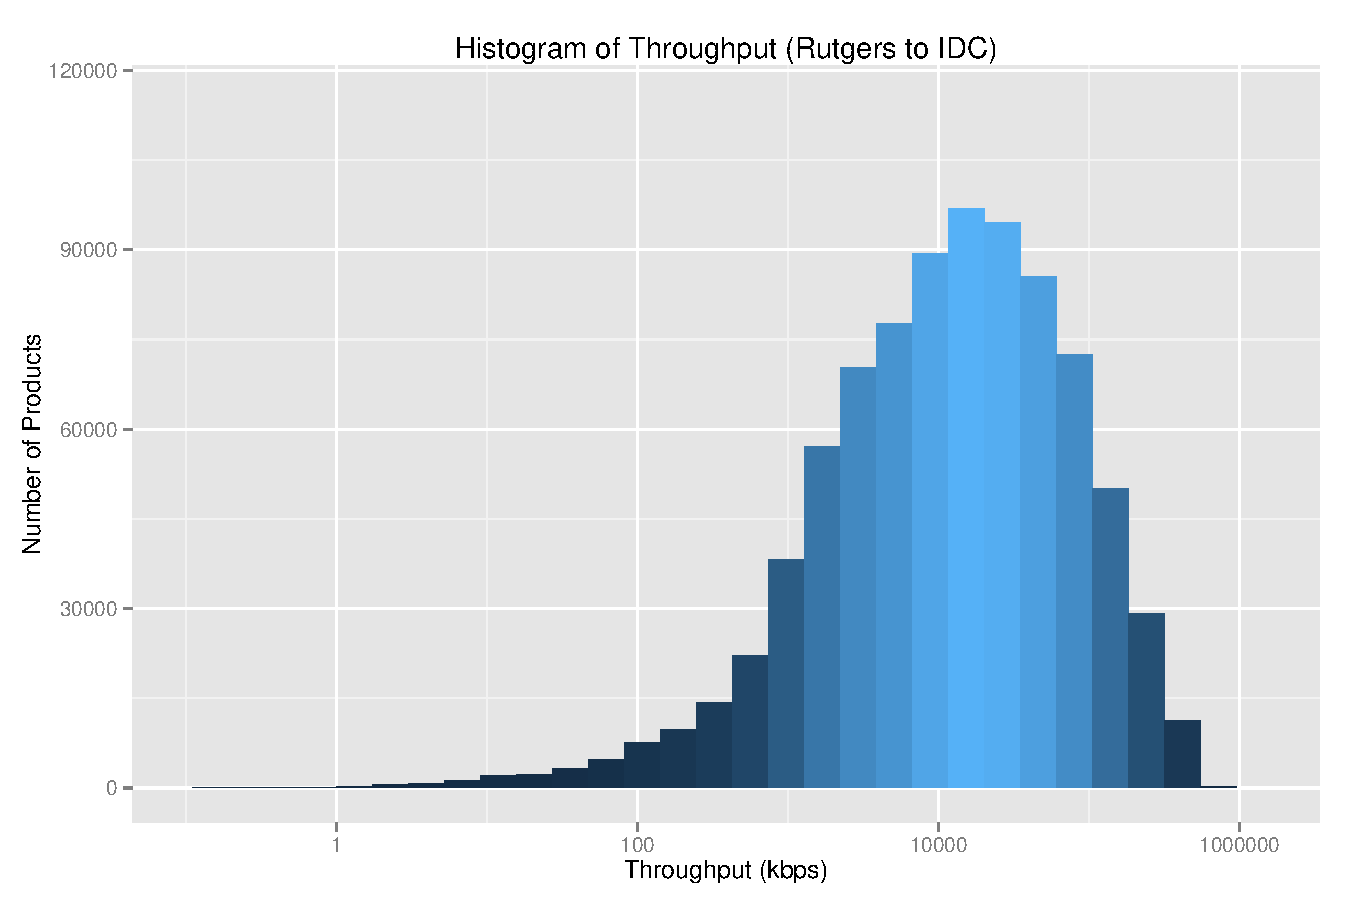
\includegraphics[width=0.9\textwidth]{figures/1-day-1-rcv-single-product-throughput.pdf}
\caption{Histogram of single file throughput measurements for LDM6 transfer from Rutgers FDT to UVA IDC}
\label{fig:single-file-throughput}
\end{subfigure}
\begin{subfigure}[b]{0.47\textwidth}
\centering
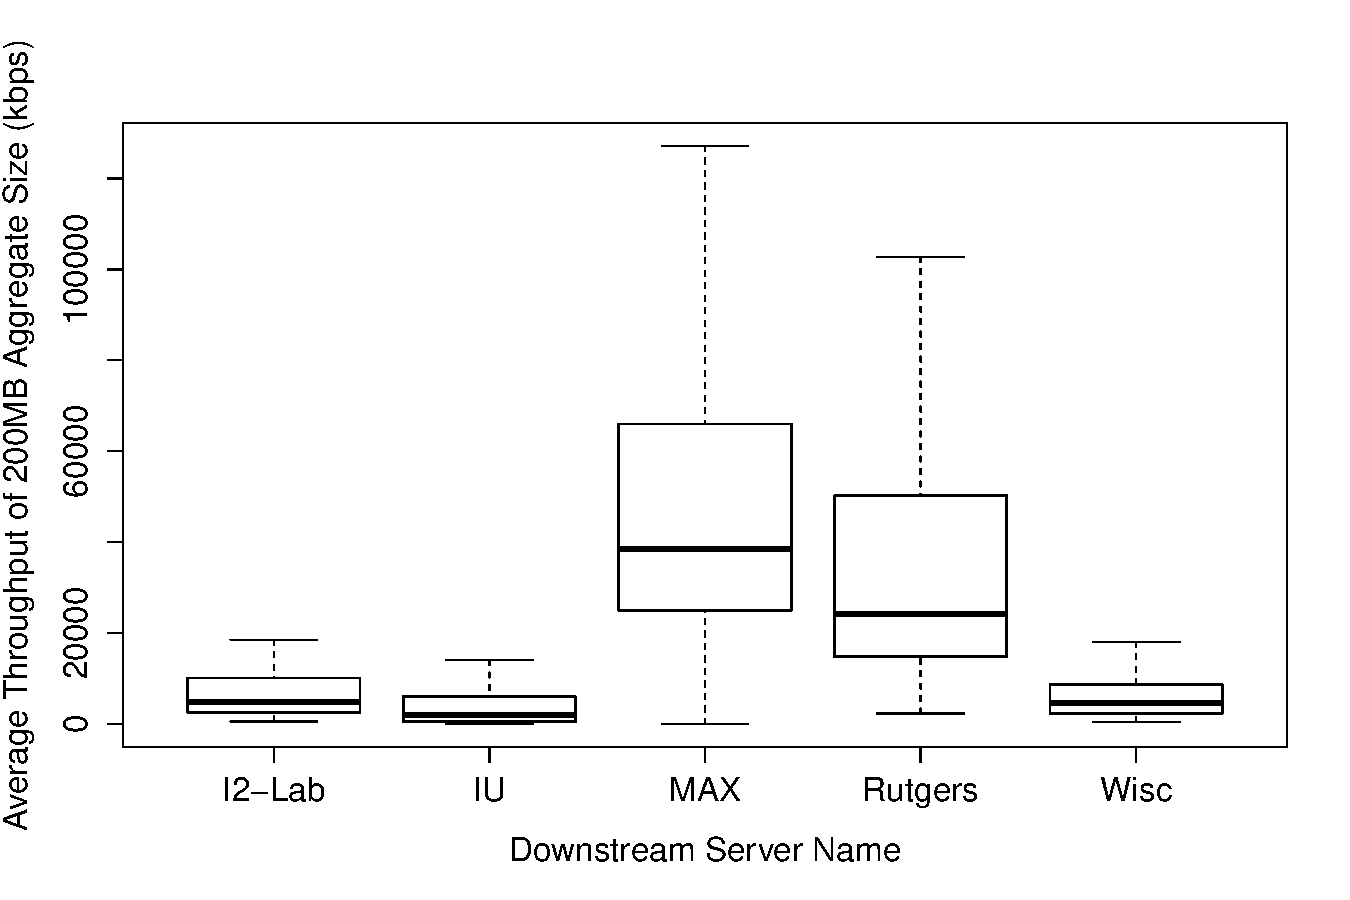
\includegraphics[width=0.9\textwidth]{figures/DYNESThroughput_IP_Path.pdf}
\caption{Sender at UVA; Receivers at the five listed sites}
\label{fig:DYNES-throughput}
\end{subfigure}
\caption{LDM-6 throughput in DYNES experiments}
\label{fig:marking-rate-effects}
\end{figure*}

\begin{figure*}
\centering
\begin{subfigure}[b]{0.47\textwidth}
\centering
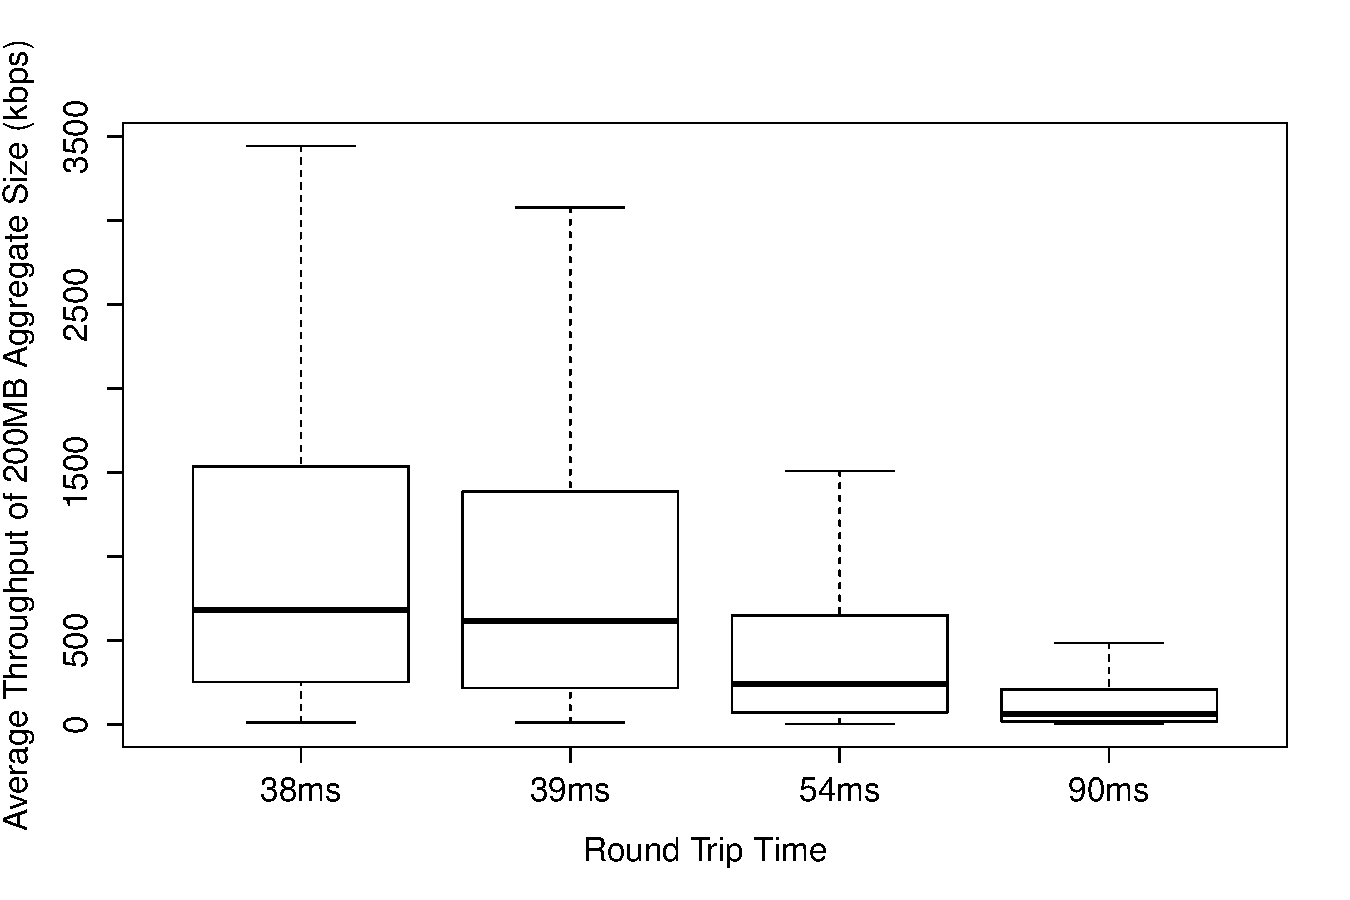
\includegraphics[width=0.9\textwidth]{figures/GENI_Throughput_BoxPlots_RTT.pdf}
\caption{Boxplots comparing aggregate throughput on paths to 4 receivers}
\label{fig:GENI-4-rcv-boxplots}
\end{subfigure}
\begin{subfigure}[b]{0.47\textwidth}
\centering
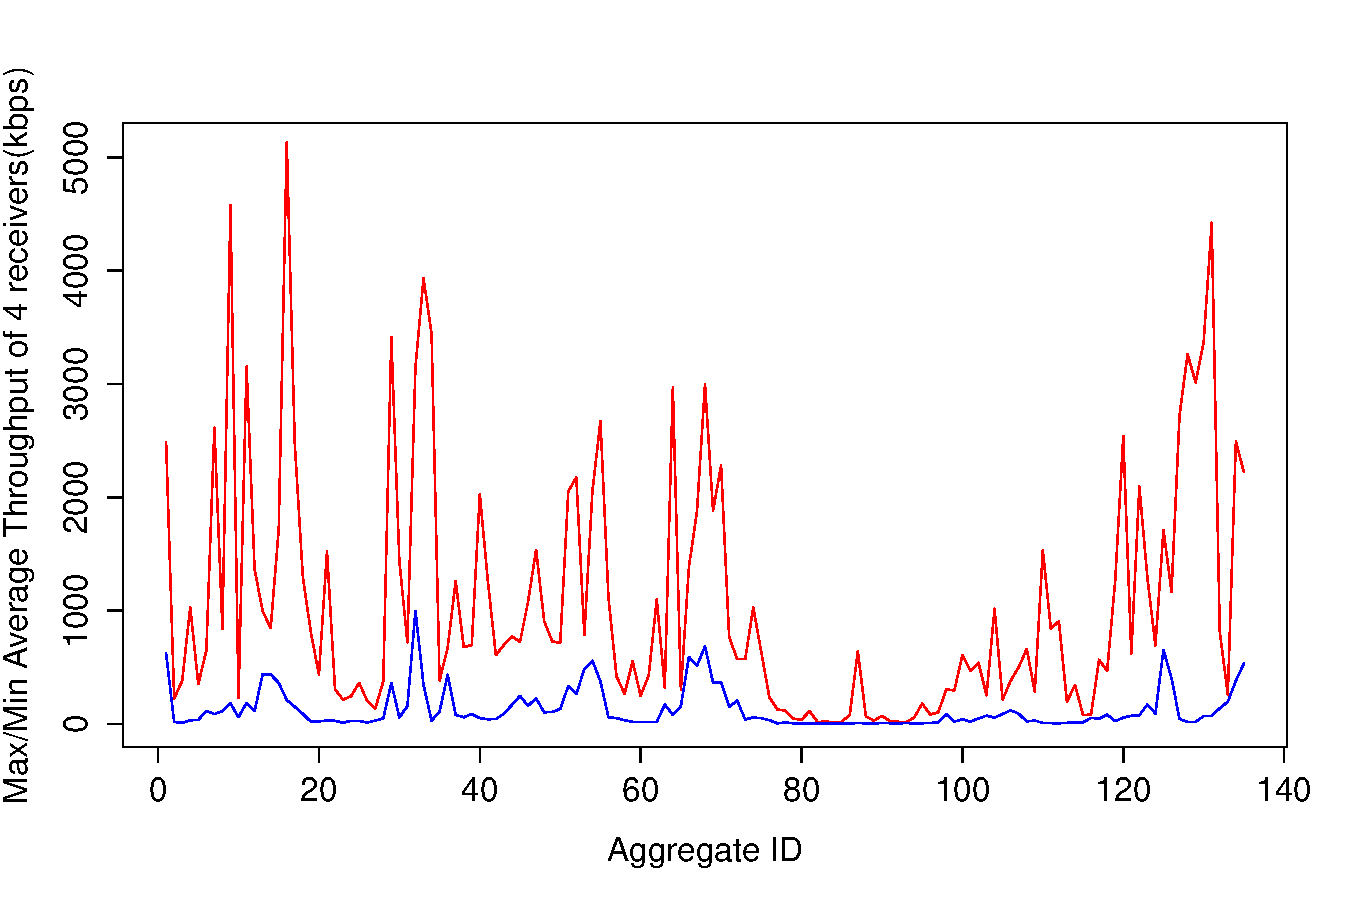
\includegraphics[width=0.9\textwidth]{figures/GENI_Throughput_vs_AggregateID.pdf}
\caption{Min and Max aggregate throughput among the four paths}
\label{fig:min-max-throughput-GENI-LDM6}
\end{subfigure}
\caption{LDM-6 throughput in GENI experiments}
\label{fig:GENI-LDM6}
\end{figure*}

Fig.~\ref{fig:GENI-LDM6} shows the the aggregate throughput measurements obtained in the GENI
experiments. Fig. ~\ref{fig:GENI-4-rcv-boxplots} compares the aggregate throughput on the paths
to 4 receivers. The RTTs on the paths from  UFL (sender) to the receivers at UMass, WSU, TAMU, and OSF, were 38, 39, 54 and 90 ms, respectively. Since CTCP was used in these GENI experiments, we did not expect a dependency on RTT.
However, the mean data product size is 65 KB for NGRID, and with the 20 Mbps sending/path rate, the mean transmission delay for products in each aggregate is only 26 ms. Thus, the RTT lowers the average throughput significantly.

Fig.~\ref{fig:min-max-throughput-GENI-LDM6} shows the minimum and maximum throughput for each aggregate
from the measurements obtained for the four paths. These results show that there is significant dependence of
the aggregate throughput on the inter-arrival times and sizes for files within each aggregate.

With respect to resource requirements, we found that the CPU usage at the sender host was 0.4\% 
when there were 4 receivers, and the usage increased linearly with the number of receivers. We are currently generating the bandwidth usage results.

\subsection{LDM CPU usage}

\subsection{LDM6 throughput for constant aggregate size, from UCAR to UVA}

\subsection{LDM Measurement of Packet loss}

\section{TCP restart measurement}

\section{Topology changing of IDD feedtypes}
\subsection{Experimental setup}
Steve setup a cron job at \emph{uni16.unidata.ucar.edu} which is one of the LDM upstream servers, the cron job executes a uldbsend command every hours to send uldbutil report to \emph{fdt-uva.dynes.virginia.edu}.

At UVA FDT site, two configuration file, ldmd.conf and pqact.conf need to be set, the detail setup is in \emph{https://github.com/XiangJi/CC-NIE-LDM/tree/master/uldbutil}. These configurations will make sure UVA FDT hosts can receive any data from UCAR servers and save the data as file locally. 

\subsection{uldbutil report}
uldbutil (Upstream LDM database utility) report provides the subscribers information for that hosts. Sample entry like: $12948 6 feeder awipsops.nsstc.uah.edu$ $20160106205353.878 TS_ENDT (CONDUIT,  .*) primary$ shows that the subscription instance 12948 whose hostname is \emph{awipsops.nsstc.uah.edu} using LDM 6 requested CONDUIT feedtype data from 20160106205353.878.

\subsection{Scripts for tracking the receivers changing for Top 5 feedtypes}
A Python script is written for counting how many receivers are requesting Top 5 feedtypes from the uldbutil report and writing the results into a csv file. This program will be executed every hour for tracking how do the subscribers change.

\section{Results}
\begin{figure*}[htb!]
\centering 
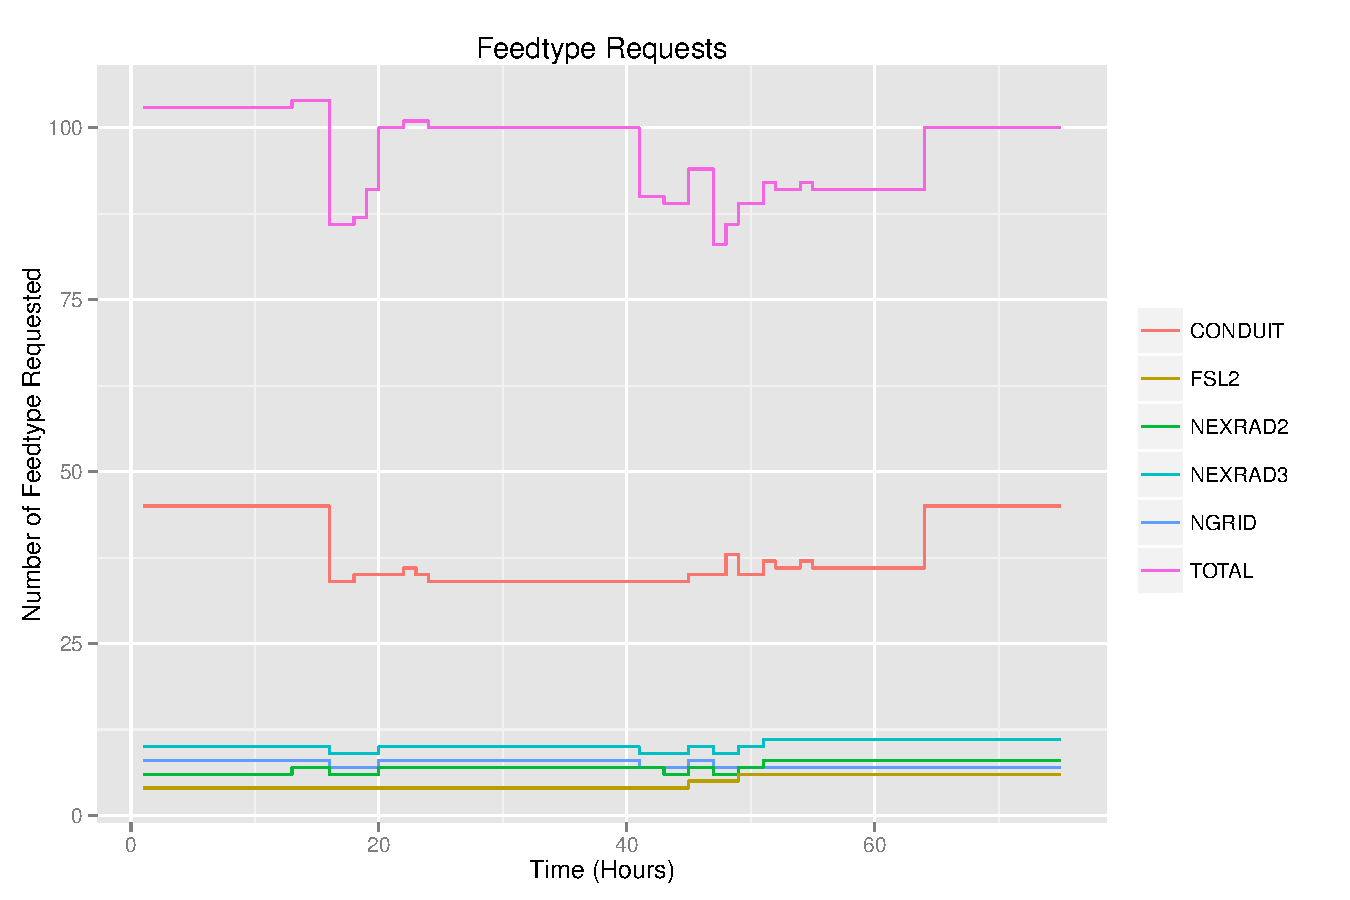
\includegraphics[width=0.96\textwidth]{figures/uldb_track.pdf}
\caption{Tracking subscibers for Top 5 feedtypes, number of subscibers for each feedtype}
\label{fig:uldb}
\end{figure*}

Fig.~\ref{fig:uldb} shows that how do the subscribers number change in 3 days for Top 5 feedtypes. It indicates that CONDUIT is the major feedtype the weather data research institutions are subscribing. By using the uldbutil report, we can record which receiver is requesting which feedtypes data. This report can inform the LDM control to use OESS to change the OpenFlow path with corresponding endpoints and bandwidth need to be reserved.  



\section{Conclusions}
The monitoring tools have been developed, shell scripts have been coded, and Python and R programs have been implemented to execute a systematic set of experiments on GENI and LDM to obtain measurements for throughput and resource
consumption. Preliminary results have been obtained on both testbeds. Rutgers (Slezak and Decker)
are working with us on LDM6 experiments, and U. Wisc (Robaidek) is working with us on LDM7 testing and evaluation. Rutgers will also test LDM7.